\section{问题三的建模与求解：多维因素分组与最佳时点}

\subsection{多维因素分析}

Y 染色体浓度达标时间除受 BMI 影响外，还受身高、体重、年龄等因素影响。由于 BMI、体重、身高三者高度共线（$\text{BMI}=\text{体重}/\text{身高}^2$），多重线性回归中单个系数不显著，故采用随机森林度量各因素的重要性（图~\ref{fig:q3_imp}）。

\begin{figure}[H]
  \centering
  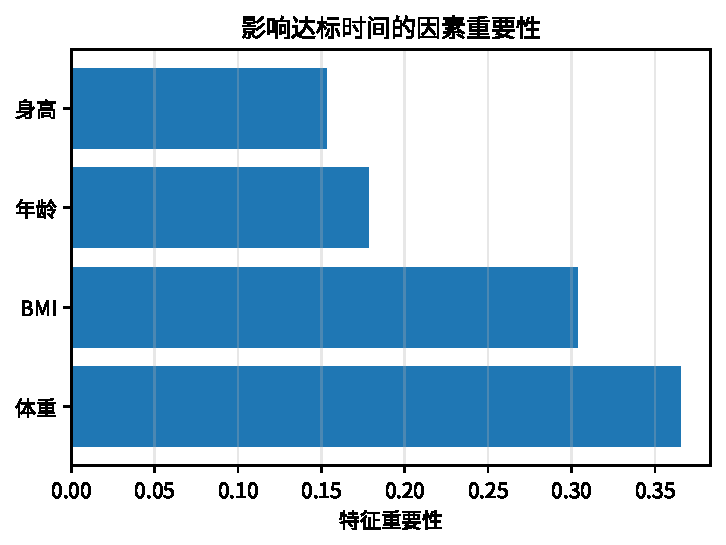
\includegraphics[width=0.6\textwidth]{../figures/fig3_1_feature_importance.pdf}
  \caption{影响达标时间的因素重要性}
  \label{fig:q3_imp}
\end{figure}

\begin{center}
\begin{tabular}{ccccc}
\toprule
\textbf{因素} & 体重 & BMI & 年龄 & 身高 \\
\midrule
\textbf{重要性} & 0.365 & 0.303 & 0.179 & 0.153 \\
\bottomrule
\end{tabular}
\captionof{table}{达标时间影响因素重要性}
\label{tab:q3_imp}
\end{center}

体重与 BMI（其衍生量）是影响达标时间的主要因素，年龄次之，身高影响最小。

\subsection{多维聚类分组}

对标准化后的特征（BMI、体重、身高、年龄）做 K-means 聚类（$K=4$），得到四组，并计算每组的最佳时点（90\% 可靠达标）：

\begin{center}
\begin{tabular}{cccccc}
\toprule
\textbf{分组} & \textbf{孕妇数} & \textbf{BMI 均值} & \textbf{体重均值} & \textbf{达标比例} & \textbf{最佳时点} \\
\midrule
组1 & 89 & 31.6 & 83.6 & 100\% & 14.5 周 \\
组2 & 61 & 32.0 & 82.9 & 100\% & 16.6 周 \\
组4 & 67 & 30.4 & 73.6 & 100\% & 16.0 周 \\
组3 & 50 & 36.4 & 99.8 & 100\% & 20.2 周 \\
\bottomrule
\end{tabular}
\captionof{table}{多维聚类分组及最佳时点}
\label{tab:q3}
\end{center}

由表~\ref{tab:q3}，BMI 与体重最高的组 3（BMI$\approx36.4$，体重$\approx99.8$）最佳时点最晚（20.2 周），BMI 最低的组 1 最早（14.5 周），与问题二结论方向一致。各组最佳时点如图~\ref{fig:q3_timing} 所示。

\begin{figure}[H]
  \centering
  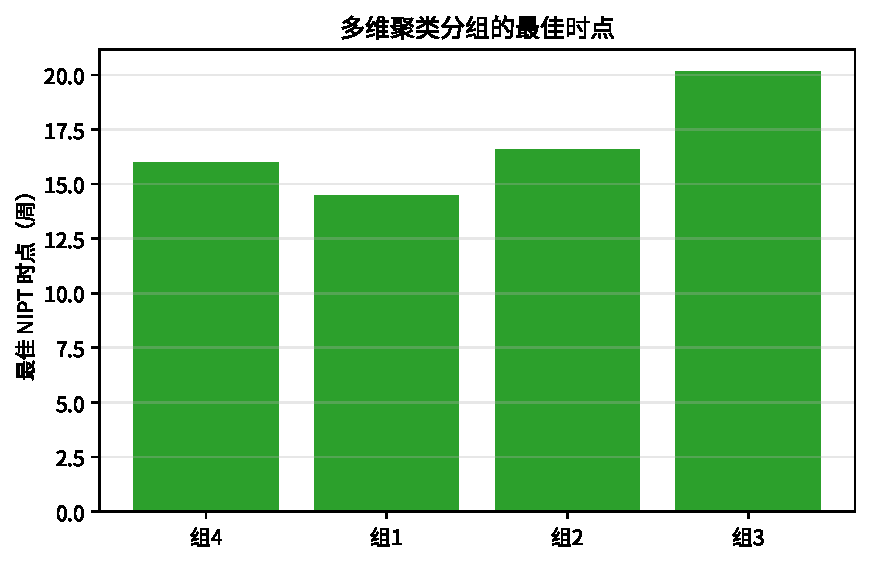
\includegraphics[width=0.68\textwidth]{../figures/fig3_2_cluster_timing.pdf}
  \caption{多维聚类分组的最佳 NIPT 时点}
  \label{fig:q3_timing}
\end{figure}

\subsection{与问题二的对比}

以组内达标时间标准差之和度量分组同质性：多维聚类为 37.12，优于仅按 BMI 分组的 40.44，说明引入身高、体重、年龄能改善组内同质性，使同一组内的孕妇在达标时间上更接近，从而各组最佳时点更具代表性。

检测误差的影响与问题二一致：误差每增加约 0.005，最佳时点后移约 2 周。综合来看，问题三通过引入多维因素细化了分组，使最佳时点的设定更贴合个体差异，进一步降低了潜在风险。
